\section{Finite Difference Method}

The finite difference method (FDM) is a numerical method used to find an approximate 
solution to differential equations. It works by creating a discrete approximation 
of the derivative with a finite difference approximation and using this approximation
to write the differential equation as a system of linear equations.

\subsection{Finite Difference}

There are three different finite difference approximations.

\begin{itemize}
	\item Forward difference, $u'(x) \approx \frac{u(x+h) - u(x)}{h}$
	\item Backward difference, $u'(x) \approx \frac{u(x) - u(x - h)}{h}$
	\item Central difference, $u'(x) \approx \frac{u(x + h) - u(x - h)}{2h}$
\end{itemize}

The forward and backward difference are first order approximations, since the
error in the approximation is $O(h)$. The central difference is a second order
approximation because the error is $O(h^2)$.

The second derivative can be approximated by applying a finite difference
approximation twice. Applying the central difference approximation to the second
derivative gives the following expression:

$$ u''(x) \approx \frac{u'(x + \frac{h}{2}) - u'(x - \frac{h}{2})}{h} $$

Another central difference approximation is applied to $u'(x + \frac{h}{2})$ and
$u'(x - \frac{h}{2})$. This results in the following finite difference
approximation for the second derivative:

$$u''(x) \approx \frac{u(x+h) - 2u(x) + u(x-h)}{h^2}$$

When applied to equations of higher dimensions it becomes necessary to choose a
value for h for each dimension.

$$(\pTwo{x} + \pTwo{y} + \pTwo{z}) u(x, y, z) = \frac{\partial^2 u(x, y, z)}{\partial^2 x} 
+ \frac{\partial^2 u(x, y, z)}{\partial^2 y} + \frac{\partial^2 u(x, y, z)}{\partial^2 z}$$

$$\frac{\partial^2 u(x, y, z)}{\partial^2 x} \approx \frac{u(x+h_x, y, z) - 2u(x, y, z) + u(x-h_x, y, z)}{h_x^2}$$

$$\frac{\partial^2 u(x, y, z)}{\partial^2 y} \approx \frac{u(x, y+h_y, z) - 2u(x, y, z) + u(x, y-h_y, z)}{h_y^2}$$

$$\frac{\partial^2 u(x, y, z)}{\partial^2 z} \approx \frac{u(x, y, z+h_z) - 2u(x, y, z) + u(x, y, z-h_z)}{h_z^2}$$

This is also known as the 7-point stencil as illustrated in figure \ref{fig:7ps}.

\begin{figure}[ht]
	\center
	
\includegraphics[width=0.5\textwidth]{images/7_point_stencil}
	\caption{7-point stencil}
	\label{fig:7ps}
\end{figure}

\subsection{Discrete Poisson Equation}

To apply the finite difference method to the Poisson equation with Dirichlet 
boundary conditions, the problem domain is sampled in a finite number of points. 
The distance between the sample points, $h$, is the same as the fixed $h$ in the finite
difference method. Lets consider the two-dimensional Poisson equation $\nabla^2
u(x, y) = f(x, y)$. We use the central difference approximation to sample
$\nabla^2 u(x, y)$ at $n+1$ points in the $x$ direction and $n+1$ points in $y$
direction. We assume the dimensions of the domain goes from $0$ to $1$. The discretized 
grid is illustrated in figure \ref{fig:discgrid}.

\begin{figure}[ht]
	\center
	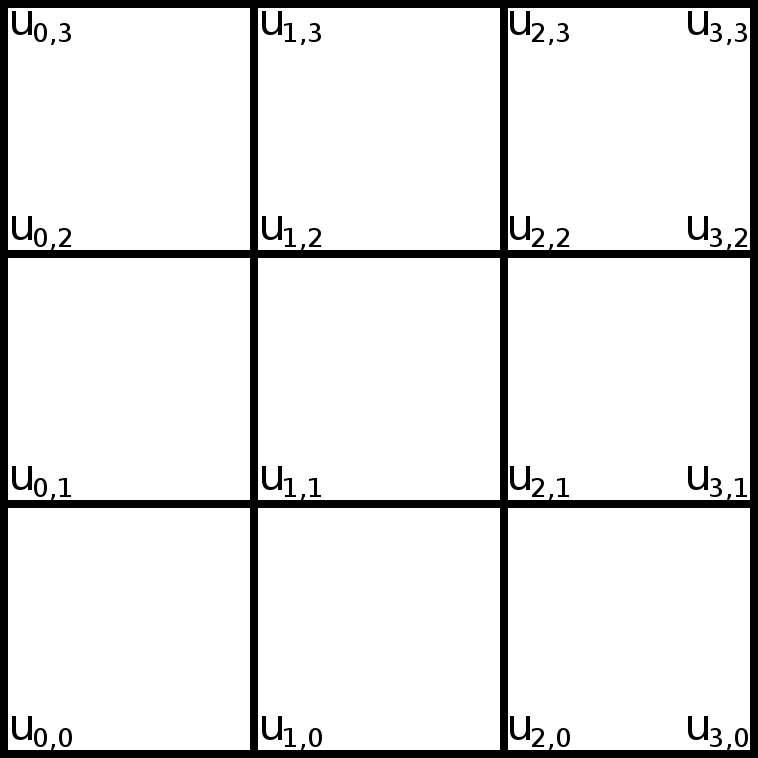
\includegraphics[width=0.6\textwidth]{images/2d_poisson_ex}
	\caption{Discretized grid with $n = 3$}
	\label{fig:discgrid}
\end{figure}

This gives $(n-1)^2$ internal points and the remaining points are boundary
points that have their values specified by the boundary conditions. The total
number of unknowns are therefore $N = (n-1)^2$.

$$h = \frac{1}{n}$$
$$x_i = ih, ~~~~ i = 0, 1, \dots, n$$
$$y_j = jh, ~~~~ j = 0, 1, \dots, n$$

We use $u_{i,j}$ as shorthand notation for the of the value of $u(x_i, y_j)$ and
$f_{i,j}$ for $f(x_i, y_j)$.

$$ (\nabla^2 u)_{ij} \approx \frac{u_{i+1,j} + u_{i,j+1} - 4u_{i,j} + u_{i-1,j} + u_{i,j-1}}{h^2} = f_{i,j} $$
$$ u_{i+1,j} + u_{i,j+1} - 4u_{i,j} + u_{i-1,j} + u_{i,j-1} = h^2 f_{i,j} $$

This creates a system of linear equations, that can be written on matrix form as
follows.

$$Ax = b$$

To create this linear system we have to create a global order for the
internal nodes to create the $x$ vector of unknowns. We use the natural
order, which means that we list the nodes along the $x$ direction first.

$$x_k = u_{i,j}, ~ k = (i-1) + (n-1) \cdot (j-1), ~ i, j = 1, 2, \dots, n-1$$

We can then assemble the matrix $A$.

$$
A = \begin{bmatrix}
 B & I & 0 & \cdots & 0 \\
 I & B & I &   & \vdots \\
 \vdots &   & \ddots &   & \vdots \\
 \vdots &   &   & \ddots & \vdots \\
 0 & \cdots & \cdots & I & B 
\end{bmatrix}
 ~ where ~ 
B = \begin{bmatrix}
-4 & 1 & 0 & \cdots & 0 \\
 1 &-4 & 1 &   & \vdots \\
 \vdots &   & \ddots &   & \vdots \\
 \vdots &   &   & \ddots & \vdots \\
 0 & \cdots & \cdots & 1 &-4 
\end{bmatrix}
$$

$A$ is a $N \times N$ matrix, $B$ is a $(n-1) \times (n-1)$ matrix and 
$I$ is the identity matrix. Below we show how the matrix $A$ looks for 
$n$ = 3.

$$
A = \begin{bmatrix}
 -4 &  1 &  1 &  0 \\
  1 & -4 &  0 &  1 \\
  1 &  0 & -4 &  1 \\
  0 &  1 &  1 & -4
\end{bmatrix}
$$
